\subsection{Demodulation}
\label{sec:demodulation}
The transmitted signal period is the inverse of the transmitted signal frequency $f_i$. 
To obtain the \textbf{signal period}, we need to know the pixel width of strip in the received image first. 
%In \autoref{fig:rx_strip}, 
As rows of pixels are sequentially obtained with sampling period $T_r$, one cycle of square wave transmission results in a pair of bright strip and dark strip in the image. 
The sum of whole widths is given by
\begin{equation}
W= \frac{1}{f_i T_r} \qquad \textrm{.}
\label{eq:widthtofreq}
\end{equation}

% \begin{figure}[!t]
% 	\centering
% 	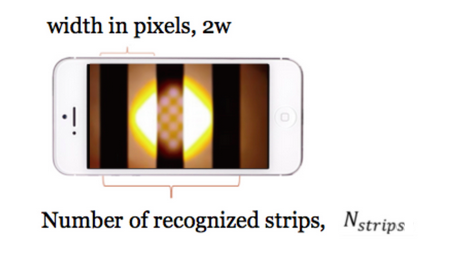
\includegraphics[scale=0.5]{fig/strip4.png}
% 	\caption{Received strips: w pixel}
% 	\label{fig:rx_strip}
% \end{figure}
\begin{figure}[!t]
\centering
  \begin{subfigure}[h]{0.12\textwidth}
  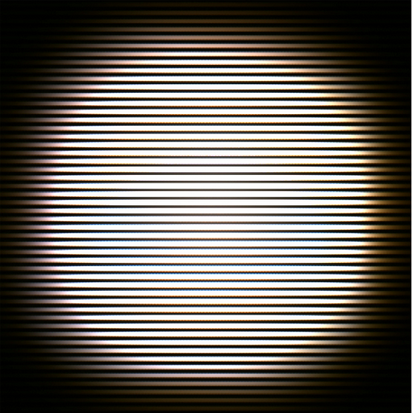
\includegraphics[width=\textwidth]{fig/strip1.png}
  \caption{8000 Hz}
  \end{subfigure}
  ~ 
  \begin{subfigure}[h]{0.12\textwidth}
  
\includegraphics[width=\textwidth]{fig/strip2.png}
  \caption{4000 Hz}
  \end{subfigure}
  ~ 
  \begin{subfigure}[h]{0.12\textwidth}
  
\includegraphics[width=\textwidth]{fig/strip3.png}
  \caption{2000 Hz}
  \end{subfigure}
\caption{Received images of different transmitting frequencies.}
\label{fig:freq_strip}
\end{figure}

Note that the width of the bright strip could be larger than the width of the dark strip in the image. This is due to blooming, the overflow of charge from a saturated pixel into its neighboring pixel~\cite{el2005cmos}. We thus consider the widths of the bright strip and the dark strip together in the calculation, to average out the effect. Since $W$ might not be an integer, averaging the observed widths over a large image area would help to improve the accuracy of the estimate of the width. Then, the transmitted period $1/f_i$ can be calculated with \autoref{eq:widthtofreq}. 

To have a more robust method to accurately determine the period of the signal, i.e., the average width of a pair of bright and dark strips in the image, we modified a well-known pitch detection algorithm (PDA), YIN~\cite{de2002yin}, that is originally designed to determine the fundamental frequency of a segment of audio signal in speech or music. We chose to use a method that operates in time domain, so that computationally expensive Fourier Transform operation can be avoided. 

We start by summing up all pixels in each row
\begin{equation}
	I[y]=\sum^{X_{\max}}_{x=1} I[x][y] \qquad \textrm{,}
\end{equation}
obtaining a one-dimensional signal, where $I[x][y]$ is the intensity (luminance)\footnote{If the obtained image is in RGB instead of grayscale, it needs to be converted to obtain the luminance information.} of the pixel at location $(x,y)$ in the received image. This operation uses pixels in different columns for redundancy, averaging out noises that exists in different columns of pixel. 

To find the period of the periodic signal presented in $I[y]$, a difference function may be constructed:
\begin{equation}
	d_\Delta(\delta)=\sum^{H/2-1}_{y=1} (I[y] - I[y+\delta])^2
\end{equation}
and we search for the values of $\delta$ that are closest to zero. Note that $\delta$ represents both the shift in space in number of pixels and the shift in time in multiples of read-out time of the camera. As pointed out in~\cite{de2002yin}, using the difference function instead of the standard autocorrelation function (ACF) can avoid a large portion of the error caused by change of amplitudes in the signal, causing by the change of luminance in different rows of pixels. An added advantage is that subtraction is computationally more efficient than multiplication. 

Another possible source of error happens at small $\delta$ values, since when $\delta<\frac{1}{f T_r}$, the difference function could produce a large value due to the fact that we use square waves - there is no significant change of signal amplitude except at the sharp transitions. We instead use cumulative mean normalized difference function (CMNDF)~\cite{de2002yin} to mitigate this problem:
\begin{equation}
	d_\Delta'(\delta) =\begin{cases} 1, & \textrm{if\;} \delta=\{0,1\} \\
	d_\Delta(\delta) / \left [ (1/\delta) \sum^\delta_{j=1} d_\Delta(j) \right ] & \textrm{otherwise.} \end{cases}
\end{equation}

The function now starts from $1$ at $\delta=0$ and remains large with small $\delta$ values, and only drops below $1$ when $d_\Delta'(\delta)$ falls below average. The smallest local minimum in $d_\Delta'(0 \leq \delta \leq H/2-1)$ is then located and serves as the period estimate of the received signal.  

Using CMNDF, the system can determine the period of the transmitted signal with a resolution of read-out time. However, as the period of the signal is not always an integer multiple of the read-out time, i.e., the sampling period, the output could results in error up to half of the read-out time. We again resort to the method proposed in~\cite{de2002yin} - to use parabolic interpolation to estimate the location of the actual minimum that could exist between samples. Assuming that $\hat{\delta}$ is the integer value that corresponds to the smallest minimum in $d_\Delta'(\delta)$, this method only needs three function values, $y_{-1}=d_\Delta'(\hat{\delta}-1)$, $y_{0}=d_\Delta'(\hat{\delta})$, and $y_{+1}=d_\Delta'(\hat{\delta}+1)$, to determine the new estimate:
\begin{equation}
	\hat{\delta}'=\hat{\delta}+\frac{y_{+1}-y_{-1}}{2 (2 y_0 - y_{+1} - y_{-1})}
\end{equation}

With parabolic interpolation, our modified YIN algorithm can very accurately determine the period of the transmitted signal. Note that the output of the algorithm is in pixel. It can be converted back to be in unit of time by multiplying the number with $T_r$.
